\documentclass[journal,12pt,twocolumn]{IEEEtran}

\usepackage{setspace}
\usepackage{gensymb}
\singlespacing
\usepackage[cmex10]{amsmath}
\usepackage{amssymb}
\usepackage{xurl}
\usepackage{tabularx}
\usepackage{amsthm}
\usepackage{comment}
\usepackage{mathrsfs}
\usepackage{txfonts}
\usepackage{stfloats}
\usepackage{bm}
\usepackage{cite}
\usepackage{cases}
\usepackage{subfig}
\usepackage{arydshln}
\usepackage{longtable}
\usepackage{multirow}

\usepackage{enumitem}
\usepackage{mathtools}
\usepackage{steinmetz}
\usepackage{tikz}
\usepackage{circuitikz}
\usepackage{verbatim}
\usepackage{tfrupee}
\usepackage[breaklinks=true]{hyperref}
\usepackage{graphicx}
\usepackage{tkz-euclide}
\usetikzlibrary{automata, positioning}
\usetikzlibrary{calc,math}
\usepackage{listings}
    \usepackage{color}                                            %%
    \usepackage{array}                                            %%
    \usepackage{longtable}                                        %%
    \usepackage{calc}                                             %%
    \usepackage{multirow}                                         %%
    \usepackage{hhline}                                           %%
    \usepackage{ifthen}                                           %%
    \usepackage{lscape}     
\usepackage{multicol}
\usepackage{chngcntr}
\usepackage{blkarray}

\DeclareMathOperator*{\Res}{Res}

\renewcommand\thesection{\arabic{section}}
\renewcommand\thesubsection{\thesection.\arabic{subsection}}
\renewcommand\thesubsubsection{\thesubsection.\arabic{subsubsection}}

\renewcommand\thesectiondis{\arabic{section}}
\renewcommand\thesubsectiondis{\thesectiondis.\arabic{subsection}}
\renewcommand\thesubsubsectiondis{\thesubsectiondis.\arabic{subsubsection}}


\hyphenation{op-tical net-works semi-conduc-tor}
\def\inputGnumericTable{}                                 %%

\lstset{
%language=C,
frame=single, 
breaklines=true,
columns=fullflexible
}
\begin{document}


\newtheorem{theorem}{Theorem}[section]
\newtheorem{problem}{Problem}
\newtheorem{proposition}{Proposition}[section]
\newtheorem{lemma}{Lemma}[section]
\newtheorem{corollary}[theorem]{Corollary}
\newtheorem{example}{Example}[section]
\newtheorem{definition}[problem]{Definition}

\newcommand{\BEQA}{\begin{eqnarray}}
\newcommand{\EEQA}{\end{eqnarray}}
\newcommand{\define}{\stackrel{\triangle}{=}}
\bibliographystyle{IEEEtran}
\raggedbottom
\setlength{\parindent}{0pt}
\providecommand{\mbf}{\mathbf}
\providecommand{\pr}[1]{\ensuremath{\Pr\left(#1\right)}}
\providecommand{\qfunc}[1]{\ensuremath{Q\left(#1\right)}}
\providecommand{\sbrak}[1]{\ensuremath{{}\left[#1\right]}}
\providecommand{\lsbrak}[1]{\ensuremath{{}\left[#1\right.}}
\providecommand{\rsbrak}[1]{\ensuremath{{}\left.#1\right]}}
\providecommand{\brak}[1]{\ensuremath{\left(#1\right)}}
\providecommand{\lbrak}[1]{\ensuremath{\left(#1\right.}}
\providecommand{\rbrak}[1]{\ensuremath{\left.#1\right)}}
\providecommand{\cbrak}[1]{\ensuremath{\left\{#1\right\}}}
\providecommand{\lcbrak}[1]{\ensuremath{\left\{#1\right.}}
\providecommand{\rcbrak}[1]{\ensuremath{\left.#1\right\}}}
\theoremstyle{remark}
\newtheorem{rem}{Remark}
\newcommand{\sgn}{\mathop{\mathrm{sgn}}}
\providecommand{\abs}[1]{\vert#1\vert}
\providecommand{\res}[1]{\Res\displaylimits_{#1}} 
\providecommand{\norm}[1]{\lVert#1\rVert}
%\providecommand{\norm}[1]{\lVert#1\rVert}
\providecommand{\mtx}[1]{\mathbf{#1}}
\providecommand{\mean}[1]{E[ #1 ]}
\providecommand{\fourier}{\overset{\mathcal{F}}{ \rightleftharpoons}}
%\providecommand{\hilbert}{\overset{\mathcal{H}}{ \rightleftharpoons}}
\providecommand{\system}{\overset{\mathcal{H}}{ \longleftrightarrow}}
	%\newcommand{\solution}[2]{\textbf{Solution:}{#1}}
\newcommand{\solution}{\noindent \textbf{Solution: }}
\newcommand{\cosec}{\,\text{cosec}\,}
\providecommand{\dec}[2]{\ensuremath{\overset{#1}{\underset{#2}{\gtrless}}}}
\newcommand{\myvec}[1]{\ensuremath{\begin{pmatrix}#1\end{pmatrix}}}
\newcommand{\mydet}[1]{\ensuremath{\begin{vmatrix}#1\end{vmatrix}}}
\newcommand*{\permcomb}[4][0mu]{{{}^{#3}\mkern#1#2_{#4}}}
\newcommand*{\perm}[1][-3mu]{\permcomb[#1]{P}}
\newcommand*{\comb}[1][-1mu]{\permcomb[#1]{C}}
\numberwithin{equation}{subsection}
\makeatletter
\@addtoreset{figure}{problem}
\makeatother
\let\StandardTheFigure\thefigure
\let\vec\mathbf
\renewcommand{\thefigure}{\theproblem}
\def\putbox#1#2#3{\makebox[0in][l]{\makebox[#1][l]{}\raisebox{\baselineskip}[0in][0in]{\raisebox{#2}[0in][0in]{#3}}}}
     \def\rightbox#1{\makebox[0in][r]{#1}}
     \def\centbox#1{\makebox[0in]{#1}}
     \def\topbox#1{\raisebox{-\baselineskip}[0in][0in]{#1}}
     \def\midbox#1{\raisebox{-0.5\baselineskip}[0in][0in]{#1}}
\vspace{3cm}
\title{\textbf{PROBABILITIY AND RANDOM VARIABLES\\ASSIGNMENT 2}}
\author{GANJI VARSHITHA - AI20BTECH11009}
\maketitle
\newpage
\bigskip
\renewcommand{\thefigure}{\arabic{figure}}
\renewcommand{\thetable}{\arabic{table}}
Download latex codes from 
%
\begin{lstlisting}
https://github.com/VARSHITHAGANJI/AI1103_Probability_Assignment/blob/main/Assignment2.tex
\end{lstlisting}
\section*{QUESTION}
\textbf{Gate EC Problem 9 }
\\
Step 1. Flip a coin twice.\\
Step 2. If the outcomes are \brak{\text{TAILS, HEADS}}
then output Y and stop.\\
Step 3. If the outcomes are either \brak{\text{HEADS,
HEADS}} or \brak{\text{HEADS, TAILS}}, then output N
and stop.\\
Step 4. If the outcomes are \brak{\text{TAILS, TAILS}},
then go to Step 1.\\
The probability that the output of the experiment is Y is (upto two decimal places) $\cdots$
\section*{SOLUTION}
Given, a fair coin is tossed is tossed two times.

Let's define a Markov chain $\{X_{n},n=0,1,2,\dots\}$, where $X_{n}\in S=\{1,2,3\}$, such that
\begin{table}[h!]
\centering
\caption{States and their notations}
\label{table:1}
\begin{tabular}{|c|c|}
    \hline
    Notation & State \\
    \hline
    $S=1$ & getting \cbrak{TT}\\[1ex]
    \hline
    $S=2$ & getting output Y\\[1ex]
    \hline
    $S=3$ & getting output N\\[1ex]
    \hline
\end{tabular}
\end{table}\\
The state transition matrix for the Markov chain is
\begin{align}
\label{eq:1}
P=\begin{blockarray}{cccccc}
&1 & 2 & 3 \\
\begin{block}{c[ccccc]}
  1 & 0.25 & 0.25 & 0.5  \\
  2 & 0 & 1 & 0 \\
  3 & 0 & 0 & 1  \\
\end{block}
\end{blockarray}
\end{align}
Clearly, the state $1$ are transient, while $2,3$ are absorbing. The standard form of a state transition matrix is
\begin{align}
\label{eq:2}
P=\begin{blockarray}{ccc}
&A & N \\
\begin{block}{c[cc]}
  A & I & O  \\
  N & R & Q \\
\end{block}
\end{blockarray}
\end{align}
where,
\begin{table}[h!]
\centering
\caption{Notations and their meanings}
\label{table:2}
\begin{tabular}{|c|c|}
    \hline
    Notation & Meaning \\
    \hline
    $A$ & All absorbing states\\[1ex]
    \hline
    $N$ & All non-absorbing states\\[1ex]
    \hline
    $I$ & Identity matrix\\[1ex]
    \hline
    $O$ & Zero matrix\\[1ex]
    \hline
    $R,Q$ & Other submatices\\[1ex]
    \hline
\end{tabular}
\end{table}
Converting \eqref{eq:1} to standard form, we get
\begin{align}
P=\begin{blockarray}{cccccc}
&2 & 3 & 1  \\
\begin{block}{c[ccccc]}
  2 & 1 & 0 & 0  \\
  3 & 0 & 1 & 0 \\
  1 & 0.25 & 0.5 & 0.25  \\
\end{block}
\end{blockarray}
\end{align}
From \eqref{eq:2},
\begin{align}
\tag{104.5}
\label{eq:r,q}
    R=\begin{bmatrix}
    0.25 & 0.5\\
    \end{bmatrix},
    Q=\begin{bmatrix}
    0.25\\
    \end{bmatrix}
\end{align}

The limiting matrix for absorbing Markov chain is
\begin{align}
\bar P=\begin{bmatrix}
    I & O\\
    FR & O\\
    \end{bmatrix}
\end{align}
where,
\begin{align}
F=(I-Q)^{-1}
\end{align}
is called the fundamental matrix of $P$. \\
On solving, we get
\begin{align}
\bar P=\begin{blockarray}{cccccc}
&2 & 3 & 1 \\
\begin{block}{c[ccccc]}
    2 & 1 & 0 & 0\\ 
    3 & 0 & 1 & 0\\ 
    1 & 0.33 & 0.17 & 0\\    
\end{block}
\end{blockarray}
\end{align}
A element $\bar p_{ij}$ of $\bar P$ denotes the absorption probability in state $j$, starting from state $i$. 
\\ Then, the absorption probability in state 2 $\brak{\text{i.e getting output Y}}$ starting from state 1 is $\bar p_{12}$.
\begin{align}
\therefore \bar p_{12}=0.33 \brak{\text{correct upto 2 decimal places}}
\end{align}



\begin{figure}[h]
\caption*{\textbf{Markov chain diagram}}
\centering

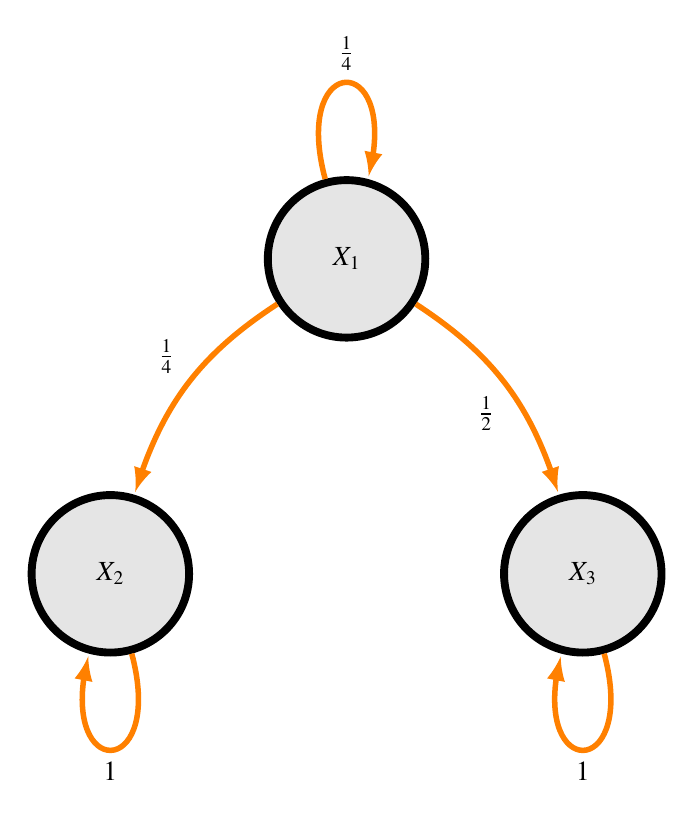
\begin{tikzpicture}

       
             % Setup the style for the states
        \tikzset{node style/.style={state, 
                                    minimum width=2cm,
                                    line width=1mm,
                                    fill=gray!20!white}}

        % Draw the states
        \node[node style] at (3, 0)      (bull)     {$X_{1}$};
        \node[node style] at (0, -4)      (bear)     {$X_{2}$};
        \node[node style] at (6, -4) (stagnant) {$X_{3}$};

        % Connect the states with arrows
        \draw[every loop,
              auto=right,
              line width=0.7mm,
              >=latex,
              draw=orange,
              fill=orange]
           (bull)     edge[bend left=20]            node {$\frac{1}{2}$} (stagnant)
            (bull)     edge[bend right=20] node {$\frac{1}{4}$} (bear)
            
            
            (bull) edge[loop above]             node  {$\frac{1}{4}$} (bull)
            (bear) edge[loop below]             node  {1} (bear)
            (stagnant) edge[loop below]             node  {1} (stagnant);

    \end{tikzpicture}
\end{figure}
\end{document}
